\documentclass[12pt]{article}
\usepackage{newtxtext}
\usepackage[T1]{fontenc}
\usepackage{etoolbox}



\makeatletter
%\patchcmd{<cmd>}{<search>}{<replace>}{<success>}{<failure>}
\patchcmd{\@makechapterhead}{\huge}{\large}{}{}% for \chapter
\patchcmd{\@makechapterhead}{\Huge}{\large}{}{}% for \chapter
\patchcmd{\@makeschapterhead}{\Huge}{\large}{}{}% for \chapter*
\patchcmd{\@makeschapterhead}{\HUGE}{\large}{}{}
\makeatother

\usepackage[top=1in, bottom=1in, left= 1in, right=1in]{geometry}
\usepackage{amsmath}
\usepackage{enumitem}
\usepackage[english]{babel}
\usepackage{hyperref}
\usepackage[utf8]{inputenc}
% \usepackage{xcolor}
\usepackage[autostyle]{csquotes}
\usepackage{graphicx}
\usepackage[stable]{footmisc}
\usepackage{subfig}
\usepackage{listings}
\usepackage{floatrow}
\usepackage{textcomp}
\usepackage{tabulary}
\newcolumntype{K}[1]{>{\centering\arraybackslash}p{#1}}
\usepackage[table]{xcolor}
\newfloatcommand{capbtabbox}{table}[][\FBwidth]
\usepackage{framed}

\definecolor{codegreen}{rgb}{0,0.6,0}
\definecolor{codegray}{rgb}{0.5,0.5,0.5}
\definecolor{codepurple}{rgb}{0.58,0,0.82}
\definecolor{backcolour}{rgb}{0.95,0.95,0.92}

\lstdefinestyle{mystyle}{
    backgroundcolor=\color{backcolour},   
    commentstyle=\color{codegreen},
    keywordstyle=\color{magenta},
    numberstyle=\tiny\color{codegray},
    stringstyle=\color{codepurple},
    basicstyle=\ttfamily\footnotesize,
    breakatwhitespace=false,         
    breaklines=true,                 
    captionpos=b,                    
    keepspaces=true,                 
    numbers=left,                    
    numbersep=5pt,                  
    showspaces=false,                
    showstringspaces=false,
    showtabs=false,                  
    tabsize=2
}
\lstset{style=mystyle}
\setlength{\parindent}{4em}
\setlength{\parskip}{1em}
\setcounter{tocdepth}{3} % Show sections

\usepackage{pgf}
\usepackage{pgfpages}

\pgfpagesdeclarelayout{boxed}
{
  \edef\pgfpageoptionborder{2pt}
}
{
  \pgfpagesphysicalpageoptions
  {%
    logical pages=1,%
  }
  \pgfpageslogicalpageoptions{1}
  {
    border code=\pgfsetlinewidth{2pt}\pgfstroke,%
    border shrink=\pgfpageoptionborder,%
    resized width=.95\pgfphysicalwidth,%
    resized height=.95\pgfphysicalheight,%
    center=\pgfpoint{.5\pgfphysicalwidth}{.5\pgfphysicalheight}%
  }%
}

\pgfpagesuselayout{boxed}


%\title{}
%\author{ }
%\date{ }
\begin{document}


\begin{center}
\normalsize{A dissertation report on} \\ 
\vspace*{1em}
\Large{\textbf{\enquote{Mechanics of Orbit Using Python(MOPy)}}}\\ \vspace{0.5em}
\normalsize{Submitted to}\\ \vspace{1em}

\includegraphics[scale=0.7]{AU.png}\\ \vspace{1em}
\normalsize{In partial fulfilment of the requirements for the award of degree} \\
\Large{\textbf{Bachelor of Technology}}\\
\Large{\textbf{In}}\\
\Large{\textbf{Aerospace Engineering}}\\ \vspace*{1em}
\normalsize Submitted by: \vspace*{1em} \\
\normalsize
\begin{tabular}{cc}
\textbf{Ramkiran L.} & \textbf{Manjunath} \\ 
17030141AE007 & 17030141AE009 \\ 
{{{\fontfamily{ptm}\selectfont
lramkiranBTECH17@ced.alliance.edu.in}}} & {{{\fontfamily{ptm}\selectfont
manjunathBTECH17@ced.alliance.edu.in}}} \vspace*{1em} \\ 
\textbf{Monisha Patel A.} & \textbf{Thoshitha R. Kumar} \\ 
17030141AE013 & 17030141AE027 \\ 
{{{\fontfamily{ptm}\selectfont
pamonishaBTECH17@ced.alliance.edu.in}}} & {{{\fontfamily{ptm}\selectfont
kuthoshithaBTECH17@ced.alliance.edu.in}}} \vspace*{1em} \\ 
\end{tabular} 
\normalsize
Under the guidance of\\
\begin{tabular}{cc}
\textbf{Prof. Gisa G.S.} & \textbf{Prof. Yadu Krishnan} \\
Assistant Professor & Assistant Professor \\
Department of Aerospace Engineering,& Department of Aerospace Engineering,\\
Alliance College of Engineering and Design, & Alliance College of Engineering and Design,\\
Alliance University & Alliance University\\
Bengaluru. & Bengaluru. \vspace*{1em} \\
\end{tabular}
\textbf{Department of Aerospace Engineering}\\
\textbf{Alliance College of Engineering and Design}\\
\textbf{Alliance University, Bengaluru - 562106} \\
\textbf{Batch - 2017-21}\\
\textbf{Year - 2021}
\end{center}
\thispagestyle{empty}
\newpage
\begin{center}

\includegraphics[scale=0.7]{AUText.png} \vspace*{2em}\\
\textbf{CERTIFICATE}
\end{center}
This is to certify that \textbf{Mr. Ramkiran L. (17030141AE007), Mr. Manjunath (17030141AE009), Ms. Monisha Patel A. (17030141AE012)} and \textbf{Ms. Thoshitha R. Kumar (17030141AE027)} students of \textbf{Aerospace Engineering, Bachelor of Technology 2017-21} batch at \textbf{Alliance College of Engineering and Design (ACED), Alliance University, Bengaluru} has completed the project report titled \textit{\textbf{\enquote{Mechanics of Orbit using Python}}} under my guidance in partial fulfillment for the award of Bachelor of Technology degree in Aerospace Engineering, Alliance University, Bangalore during the year 2020-2021. \vspace{1em}\\
\begin{center}
\begin{tabular}{K{7cm} K{0.5cm} K{7cm}}
\underline{\hspace{2.9cm}} & & \underline{\hspace{4.3cm}} \\ 
\textbf{Prof. Gisa G.S} & & \textbf{Prof. Yadu Krishnan} \vspace{1em}\\ 
Internal Guide & &  Internal Guide\\ 
Department of Aerospace Engineering & & Department of Aerospace Engineering \\
ACED, Alliance University & & ACED, Alliance University \\ 
Bengaluru & & Bengaluru \vspace{3em}\\ 
\underline{\hspace{5cm}}&&\underline{\hspace{3.5cm}}\\ 
\textbf{Prof. Velmurugarajan K.}&&\textbf{Dr. Reeba Korah}\vspace{1em} \\ 
Head of the Department&&Interim Dean \\ 
Department of Aerospace Engineering&&Department of Aerospace Engineering\\
ACED, Alliance University&&ACED, Alliance University\\ 
Bengaluru&&Bengaluru\vspace{2em}\\ 
\end{tabular} 
\end{center}
\textbf{External Viva}
\begin{center}
\begin{tabular}{c K{7cm} K{7cm}}
 & \textbf{Name of Examiners} & \textbf{Signature with date} \\
\textbf{1.} & & \\ 
&&\\
\textbf{2.} & & \\
\end{tabular}
\end{center}
\thispagestyle{empty}
\newpage
\begin{center}
\Large \textbf{DECLARATION}
\end{center}
\normalsize
\hspace{4em}We, Ramkiran L, Manjunath, Monisha Patel A, Thoshitha R. Kumar students of 8\textsuperscript{th} Semester Bachelor of Technology in Aerospace Engineering, Alliance College of Engineering and Design (ACED), Alliance University, Bengaluru, hereby declare that the entire project work entitled \enquote{\textbf{Mechanics of Orbit using Python}} is an authentic record of the work that has been carried out independently by us during final year of our B.Tech at ACED, under the esteemed guidance \textbf{Dr. Gisa G.S}, Assistant Professor, Department of Aerospace Engineering, Alliance college of Engineering and Design, Alliance University. \par

This project report is submitted in partial fulfillment of requirements for the award of the degree of Bachelor of Technology in Aerospace Engineering. The results embodied in this dissertation are original and it has not been submitted in part or full for any degree in any University. \vspace{4em}\\
\textbf{Place:} Bengaluru\\
\textbf{Date:}17/062021 \vspace{5em}\\

\begin{center}
\begin{tabular}{K{7.5cm} K{7.5cm}}
\underline{\hspace{2.5cm}} & \underline{\hspace{2.5cm}} \\ 
\textbf{Ramkiran.L} & \textbf{Manjunath} \\ 
\textbf{17030141AE007} & \textbf{17030141AE009} \vspace{3em}\\ 
\underline{\hspace{3cm}} & \underline{\hspace{4cm}} \\ 
\textbf{Monisha Patel A.} & \textbf{Thoshitha R. Kumar} \\ 
\textbf{17030141AE012} & \textbf{17030141AE027}
\end{tabular} 
\end{center}
\thispagestyle{empty}
\newpage
\begin{center}
\Large \textbf{ACKNOWLEDGEMENT}
\end{center}
\normalsize
\hspace{4em}The satisfaction that accompanies the successful completion of any task would be incomplete without the mention of the people, who are responsible for the completion of the project and who made it possible.\par

We take this opportunity to thank our beloved Interim Dean \textbf{Dr. Reeba Korah}, ACED, Alliance University, Bangalore for providing excellent academic environment in the college and her never--ending support to the B-Tech program.\par

We would like to convey our sincere gratitude to \textbf{Prof. K. Velmurugarajan}, Head of Department of Aerospace Engineering, ACED, Alliance University, Bangalore. \par

We would like to thank our internal guide \textbf{Prof. Gisa G.S}, Assistant Professor, Department of Aerospace Engineering, ACED, Alliance University, Bangalore for her support and encouragement given to carry out the project. \par

We would also like to thank our college staff members and well-wishers who directly or indirectly helped, motivated to complete this project successfully. \par

Lastly, we thank God almighty, our family, professors and friends for their constant encouragement without which this project would not have been possible.\\
\thispagestyle{empty}
\newpage
\tableofcontents
\thispagestyle{empty}
\newpage
\setcounter{page}{1}
\section{Abstract}
\hspace{4em}Orbital mechanics is the study of the motions of artificial satellites and space vehicles moving under the influence of forces. It plays a vital role in planning space missions in various aspects such as designing orbital trajectory for various missions, calculating lagrangian points etc., and can find many engineering applications  including ascent trajectories, reentry and landing, rendezvous computations, lunar and interplanetary trajectories. 

In recent years, as there is a lot of progress unfolding in space industry, many aspiring students are keen on gaining knowledge and pursue careers in space industry. As such, strong foundations of the fundamentals are required for the students for them to get ahead in the field. There are lots of tools like STK, FreeFlyer etc., for learning but these don't start from the bare minimum of the concepts. This led to the idea of developing of MOPy.

Mechanics of Orbit using Python(MOPy) is learning tool designed and developed with the purpose of introducing the core concepts of Orbital Mechanics. MOPy uses a interactive UI with tool tips and a 3D Environment with an interactive virtual universe. The 3D Environment helps the learner to visualize the concepts in a much accessible and easier way.

\section{Introduction}
\hspace{4em}MOPy, a learning tool designed to learn and practice various orbital mechanics concepts. It is designed in a way such that it can be a user-friendly tool that can be operated with ease even by the user who has very limited knowledge about the concepts of orbital mechanics. It provides users to learn about a particular concept with a brief explanation so the user can gain the theoretical knowledge required through visualizations. The sophisticated 3D environment benefits the user to visualize the fundamental concepts easily. It assists the user to verify manually calculated data. It serves as advanced virtual calculator. MOPy is an open source software with GNU-GPL v3 license\cite{lic} which anyone can use or work with. It runs on windows platforms at present.
\begin{figure}[H]
\centering

\includegraphics[scale=0.18]{mopy.png}
\caption{MOPy} \label{mopy}
\end{figure}
\subsection{List of Features}
\begin{center}
\begin{table}[H]
{\rowcolors{2}{white}{gray!50}
\begin{tabular}{c|K{7.5cm}}
\hline 
Sl. No & \textbf{Section}\\ 
\hline 
1 & Calculation of Orbital Elements\\ 
\hline 
2 & 2D and 3D orbit \\ 
\hline 
3 & Various Parameters at any given point \\ 
\hline 
4 & 2D and 3D Orbits\\ 
\hline 
5 & Calculation of Julian Day \\ 
\hline 
5 & Euler Angles\\ 
\hline 
6 & Sphere Of Influence \\ 
\hline 
7 & Sensitivity Analysis \\ 
\hline 
8 & Position of one Spacecraft w.r.t Another\\ 
\hline 
9 & Calculation of State and Velocity Vector\\ 
\hline
10 & Orbital Transfer  \\ 
\hline
\end{tabular}}
\caption{\label{tab: features}List of Features present in MOPy}
\end{table}
\end{center}
\subsection{Python Libraries Used}
\begin{enumerate}
\item \textbf{NumPy}:  This brings MATLAB like functionality of using Matrices and their operations to python. This enables us to do a lot of stuff without much hassle.
\item \textbf{SciPy} - This enables us to add many features involving more complex computing scenarios as it has features for scientific and technical computing. For example, it has different kinds of solvers for integration which we can use for solving acceleration vector equation to obtain the position vector for an orbit.
\item \textbf{Matplotlib} - This is a plotting tool that is a extension on NumPy that gives the functionality of plotting many different kinds of graph. This library is somewhat similar to the plotting feature of MATLAB.
\item Panda3D - This is a Game Engine based on C++ that takes in syntax from both C++ and Python. This provides real-time 3D visualizations and simulations based on the code.
\item \textbf{SQLite3} - The entire details of the planetary bodies like the orbital elements, planetary ephemeris and others are stored in a local database. SQLite is used as it enables the offline functionality.
\item \textbf{Qt Deisgner} - This enables MATLAB's App Designer like feature of dragging and dropping the UI elements and creating the GUI. This is based on Qt, a cross platform GUI toolkit developed by the Qt Company
\item \textbf{PyQt5 $\&$ PySide2} - These both are the python binding libraries of Qt.
\item \textbf{PyInstaller} - This library lets us convert our python code(.py) into executable file(.exe)
\end{enumerate}
\subsection{Market Research}
There are mainly two kinds of softwares.
\begin{enumerate}
\item Simulation Based programs like STK, FreeFlyer etc.,
\item Sandbox Based programs like Universe SandBox, Kerbal Space Program etc.,
\end{enumerate}
\hspace{4em}The simulation based programs are mainly used to simulate missions and solve problems based on the instance. Both the applications given in the example are used in the industry for all kinds of missions, ranging from very small scale missions that are performed by the students to complicated missions that are performed by NASA and ISRO.

The Sandbox based programs are the stuff that are run by the physics engine that are baked into it. They use a 3D visualization toolkit or engine which lets the user easily interact with the UI, and change the parameters directly from the environment.

In the analysis done by Morgan Stanley named \enquote{Investing in Space Exploration}, it is stated as - The revenue generated by the global space industry may increase to more than $\$$1 trillion by 2040. \cite{morgan}
\begin{figure}[H]
\centering
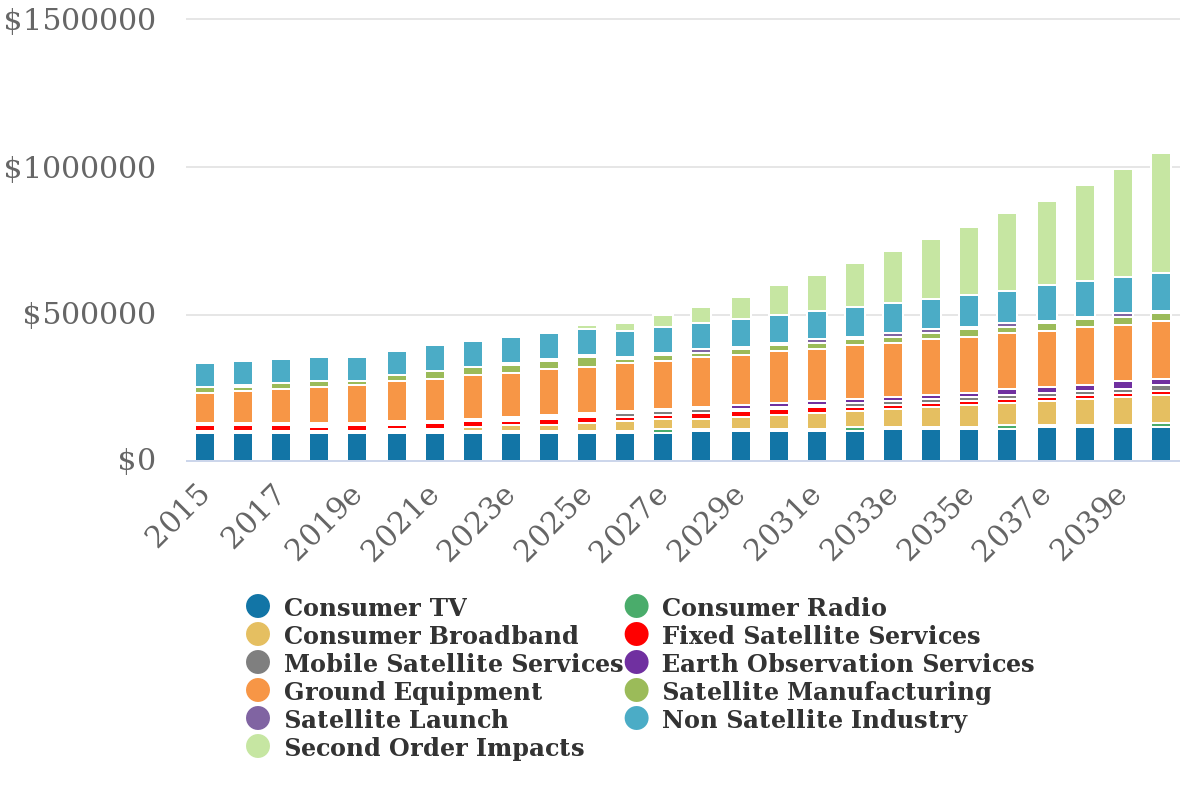
\includegraphics[scale=0.25]{morganstanley.png}
\caption{Global Market Trend according to Morgan Stanley.} \label{morgangraph}
\end{figure}
A report by Antrix and PwC, it is stated that the indian space sector can become a $\$$50 Billion industry, or about one per cent of India's projected $\$5$ Trillion economy, by 2024 from the current $\$7$ billion, according to a report by the Antrix and PwC.\cite{indiaspace}
\begin{figure}[H]
\centering
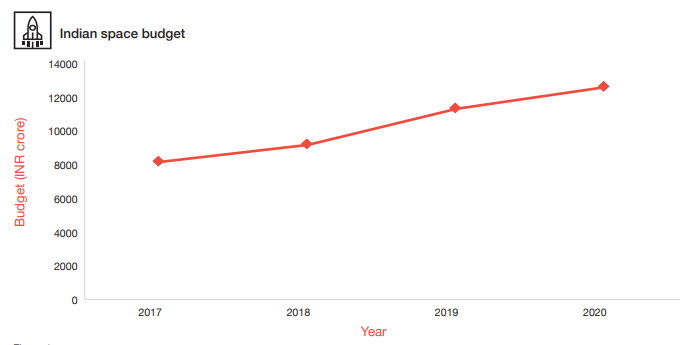
\includegraphics[scale=1]{pwc.png}
\caption{Indian Space Budget over the years.} \label{pwc}
\end{figure}
\subsection{Objective}
The development in the field of space technology is constantly increasing as shown in the aforementioned studies.
Such being the case, many students are showing interest to learn more and more about space technology and its related concepts. Considering all such possibilities, we have come up with an idea to develop a learning tool beneficial to learn more about Orbital Mechanics 
The main objectives of this project are as follows:
\begin{enumerate}
\item Design and develop a software to learn concepts and  solve Problems related orbital mechanics to understand the basics.
\item Provide a user friendly learning tool such that the user can operate even with the minimum knowledge about the concepts of orbital mechanics.
\item Help user to visualize the virtual view of the space mission.
\end{enumerate}
\subsection{Front End Development}
\subsubsection{Introduction}
Front-end development deals with the Graphical User-Interface aspect of the software. It is the key developmental process that defines how the user experiences the features we have developed. The interface between the user and the back end code is GUI. The inputs from the user is taken from the GUI. So the design must be intuitive and clear. There are many libraries that can be used to develop a GUI like PyQt, Pyside, Kivy, Tkinter, etc. In our case, we have opted for PyQt5, Pyside2 and designed GUI in Qt-Designer. Then linked the Back-End scripts through the Integrated Development Environment(IDE) by Microsoft i.e, Visual Studio Code.
\subsubsection{Home Page}
When the application opens the Home Page will load. In it, there is a Dropdown box containing all the features available, from which the user can choose which feature they want to use. When the user selects any of the features from the drop-down and clicks on the go button at the bottom, they are navigated to that screen where they can use the feature they selected. And then if they want to navigate back to the Home-Page they can click on the Home button provided at the top left corner of the screen. All the features are listed in the upper-mentioned table.
\begin{figure}[H]
\centering
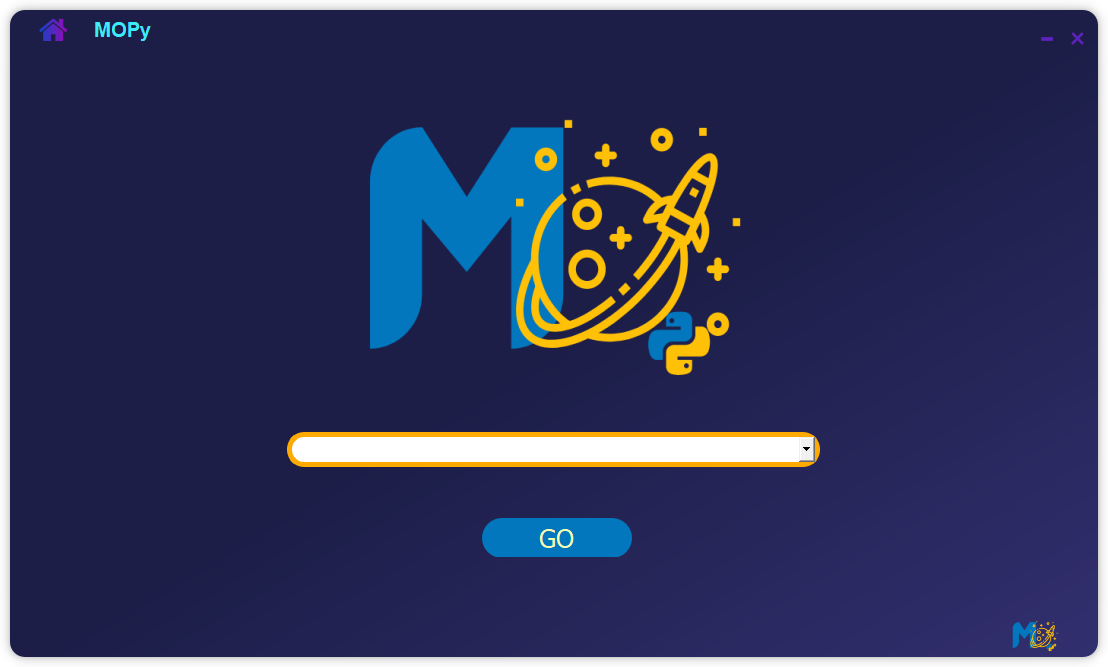
\includegraphics[scale=0.5]{homepage.png}
\caption{Home Page of MOPy} \label{home}
\end{figure}
\section{Detailed Explanation of Each Feature}
\subsection{Calculation of Orbital Elements}
\subsubsection{Theory}
\begin{figure}[H]
\begin{floatrow}
\ffigbox{%
  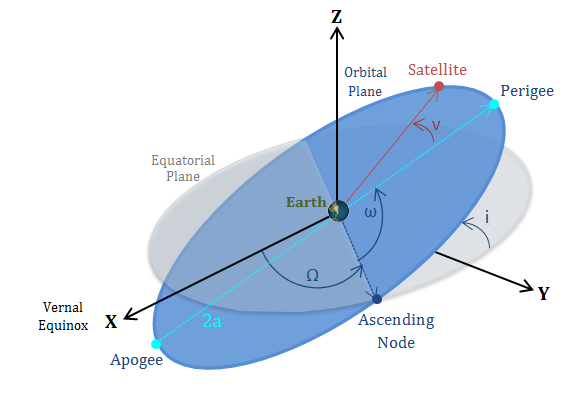
\includegraphics[scale=0.5]{COE.png}
}{
  \caption{Classical Orbital Elements} \label{COE}
}
\ffigbox{%
  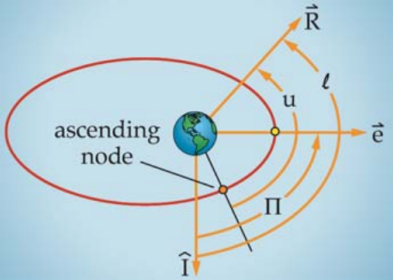
\includegraphics[scale=0.7]{AOE.png}
}{
  \caption{Alternate Orbital Elements} \label{AOE}
}
\end{floatrow}
\end{figure}
\large 
Classical Orbital Elements
\normalsize
\begin{enumerate}
\item \textbf{Semi-major Axis($a$):} This is a constant that defines the size of the orbit. In Circular it is the radius of the circle. It is the longest diameter of an ellipse.
\item \textbf{Eccentricity($e$):} This the parameter of the conic section which determines its shape. It is defined as the ratio of distance b/w two foci to the Major-axis.
\item \textbf{Inclination($e$)}: It is the tilt of the orbit w.r.t the equatorial plane, measured at ascending node. It can also be defined as the angle from $\hat{K}$ unit vector to the specific angular momentum vector $\vec{h}$.
\item \textbf{Right Ascension of Ascending Node($\Omega$):} RAAN horizontally orients the ascending node of the orbit w.r.t the Equatorial plane’s vernal equinox, measured in an equatorial plane This is not defined when the inclination is 0 or 180 degree. It lies between 0 to 360 degrees.
\item \textbf{Argument of Perigee($\omega$):} Argument of Perigee defines the orientation of the ellipse in the orbital plane, as an angle measured from the ascending node to the periapsis measure in the direction of the spacecraft’s motion. This is not defined when inclination is 0 or 180 degree or eccentricity is 0. It lies between 0 to 360 degree.
\item \textbf{True Anomaly($\nu$):} True Anomaly defines the position of the spacecraft w.r.t perigee. It’s the angle between the spacecraft and the perigee of the orbit. It lies between 0 to 360 degree. 
\end{enumerate}
\large Alternate Orbital Elements
\normalsize
\begin{enumerate}
\item \textbf{Longitude of Perigee($Pi$)} is the angle from the principle direction to perigee. This is used whenever inclination is either 0$^o$ or 180$^o$ as there is no ascending node. It's lies between $0^0$ to $360^0$. In the figure(\ref{AOE}) Longitude of perigee is represented as \enquote{$\Pi$}.
\item \textbf{True Longitude} is the angle from the principle direction to the spacecraft's position. This is used whenever there is no perigee and the the inclination is either $0^0$ or $180^0$. It's lies between $0^0$ to $360^0$. It lies between 0 to 360 degree. In the figure(\ref{AOE})True Longitude is represented as \enquote{$l$}
In the figure(\ref{AOE})True Longitude is represented as \enquote{$l$}
In the figure(\ref{AOE}) Longitude of perigee is represented as \enquote{$\Pi$}.
\end{enumerate}

\subsubsection{Algorithm}

\section{Conclusion}
\section{Future Scope}

\begin{thebibliography}{99}
	\bibitem{TB-1}{Bate, Roger R., Donald D. Muller and Jerry E. White},{ \textit{\enquote{Fundamentals Of Astrodynamics}}},{New York, NY},{ Dover Publications},{1971}.
	\bibitem{morgan}{\textit{\enquote{Space: Investing in the Final Frontier}}},{Jul, 24$^{th}$, 2020}, { Retrieved on 25$^{th}$ May 2021 from Morgan Stanley},{\href{https://www.morganstanley.com/ideas/investing-in-space}{MorganStanley.com}}
	\bibitem{indiaspace}{\textit{\enquote{Preparing to Scale New Heights: Privatisation of India's Space Sector}}}
	\bibitem{lic}{GNU General Public License version-3},{ Open Source Initiative},{\href{https://opensource.org/licenses/gpl-3.0.html}{ Open Source Initiative.org}}
	

\end{thebibliography}
\end{document}
